\section{About {\superlud}}
In this part, we describe the {\superlud} library designed for
distributed-memory pearallel computers using SPMD parallel programming model,
together with multithreading for manycore node architectures.
The library is implemented in ANSI C, using MPI~\cite{mpi-forum}
for communication, OpenMP for multithreading and CUDA for GPU.
 We have tested the code on a number of platforms, including IBM, 
Cray XE6, Cray XT7, and numerous Linux clusters.
The library includes routines to handle both real and complex matrices
in double precision.
The parallel routine names for the double-precision real version start
with letters ``pd'' (such as {\tt pdgstrf}); the parallel routine
names for double-precision complex version start with letters ``pz''
(such as {\tt pzgstrf}).

\section{Formats of the input matrices $A$ and $B$}
\label{sec:InputFormat}
We provide two input interfaces for matrices $A$ and $B$---one
is global, and the other is entirely distributed.

\subsection{Global input}\label{sec:GlobalInput}
The input matrices $A$ and $B$ are globally
available (replicated) on all the processes. The storage type for $A$
is {\NC} ({\em compressed column}), as in sequential case
(see Section~\ref{sec:rep}). The user-callable routines with this interface
all have the names ``xxxxxxx\_ABglobal''.
If there is sufficient memory, this interface is faster than
the distributed input interface described in the next section,
because the latter requires more data re-distribution at
different stages of the algorithm.

\subsection{Distributed input}\label{sec:DistInput}
Both input matrices $A$ and $B$ are distributed among all the processes.
They use the same distribution based on block rows.
That is, each process owns a block of consecutive rows of $A$ and $B$.
Each local part of sparse matrix $A$ is stored in a {\em compressed row}
format, called {\NRloc} storage type, which is defined below.
\begin{verbatim}
    typedef struct {
        int nnz_loc;  /* number of nonzeros in the local submatrix */
        int m_loc;    /* number of rows local to this process */
        int fst_row;  /* row number of the first row in the local submatrix */
        void *nzval;  /* pointer to array of nonzero values, packed by row */
        int *rowptr;  /* pointer to array of beginning of rows in nzval[] 
                         and colind[]  */
        int *colind;  /* pointer to array of column indices of the nonzeros */
    } NRformat_loc;
\end{verbatim}

Let $m_i$ be the number of rows owned by the $i$th process.
Then the global row dimension for $A$ is $nrow = \sum_{i=0}^{P-1}m_i$.
The global column dimension is $ncol$. Both $nrow$ and $ncol$
are recorded in the higher level {\tt SuperMatrix} data structure,
see Figure~\ref{fig:struct}.
The utility routine \\
{\tt dCreate\_CompRowLoc\_Matrix\_dist}
can help the user to create the structure for $A$.
The definition of this routine is
\begin{verbatim}
  void dCreate_CompRowLoc_Matrix_dist(SuperMatrix *A, int m, int n,
                                      int nnz_loc, int m_loc, int fst_row,
                                      double *nzval, int *colind, int *rowptr,
                                      Stype_t stype, Dtype_t dtype, Mtype_t mtype);
\end{verbatim}
where, the first argument is output and the rest are inputs.

The local full matrix $B$ is stored in the standard Fortran-style column
major format, with dimension $m\_loc\times nrhs$, and $ldb$ refers to
the local leading dimension in the local storage.


\section{Distributed data structures for $L$ and $U$}
\label{sec:datastruct}
We distribute both $L$ and $U$ matrices in a two-dimensional
block-cyclic fashion.
We first identify the supernode boundary based on the nonzero structure
of $L$. This supernode partition is then used as the block
partition in both row and column dimensions for both $L$ and $U$.
The size of each block is matrix dependent.
It should be clear that all the diagonal
blocks are square and full (we store zeros from $U$ in the upper triangle
of the diagonal block), whereas the off-diagonal blocks may be
rectangular and may not be full.
The matrix in~\fig{lu_2d} illustrates such a partition.
By block-cyclic mapping we mean block $(I,J)$ ($0\le I, J\le N-1$) is
mapped into the process at coordinate
\{$I\ mod\ {\tt nprow}, J\ mod\ {\tt npcol}$\}
of the ${\tt nprow}\times {\tt npcol}$ 2D process grid.
Using this mapping, a block $L(I,J)$ in the factorization is only needed
by the row of processes that own blocks in row $I$.
Similarly, a block $U(I,J)$ is only needed
by the column of processes that own blocks in column $J$.

In this 2D mapping, each block column of $L$ resides on more than
one process, namely, a column of processes. For example in~\fig{lu_2d},
the second block column of $L$ resides on the column processes \{1, 4\}.
Process 4 only owns two nonzero blocks, which are not contiguous
in the global matrix.
The schema on the right of~\fig{lu_2d} depicts the data structure
to store the nonzero blocks on a process.
Besides the numerical values stored in a Fortran-style
array {\tt nzval[]} in column major order, we need the information to
interpret the location and row subscript of each nonzero. This is stored in
an integer array {\tt index[]}, which includes the
information for the whole block column and for each individual block in it.
Note that many off-diagonal blocks are zero and hence
not stored. Neither do we store the zeros in a nonzero block.
Both lower and upper triangles of the diagonal block are stored in the
$L$ data structure.
A process owns $\lceil{N/{\tt npcol}}\rceil$ block columns of $L$, so it needs
$\lceil{N/{\tt nprow}}\rceil$ pairs of {\tt index/nzval} arrays.

For $U$, we use a row oriented storage for the block
rows owned by a process, although for the numerical values within each block
we still use column major order.  Similar to $L$, we also use a pair
of {\tt index/nzval} arrays to store a block row of $U$.
Due to asymmetry, each nonzero block in $U$ has the skyline structure
as shown in~\fig{lu_2d}
(see~\cite{superlu99} for details on the skyline structure).
Therefore, the organization of the {\tt index[]} array is different from
that for $L$, which we omit showing in the figure.

\ignore{
Since currently some steps of the algorithm (steps (1) to (3)
in~\fig{GESP_alg}) are not yet parallel,
we start with a copy of the entire matrix $A$ on each
process. 
The routine {\tt symbfact} determines the nonzero patterns of $L$
and $U$ as well as the block partition.
The routine {\tt ddistribute} uses this information to
sets up the $L$ and $U$ data structures
and load the initial values of $A$ into $L$ and $U$.
}

\begin{figure}
%\centerline{\psfig{figure=lu_2d.eps,height=2.7in,width=3.8in}}
\centering{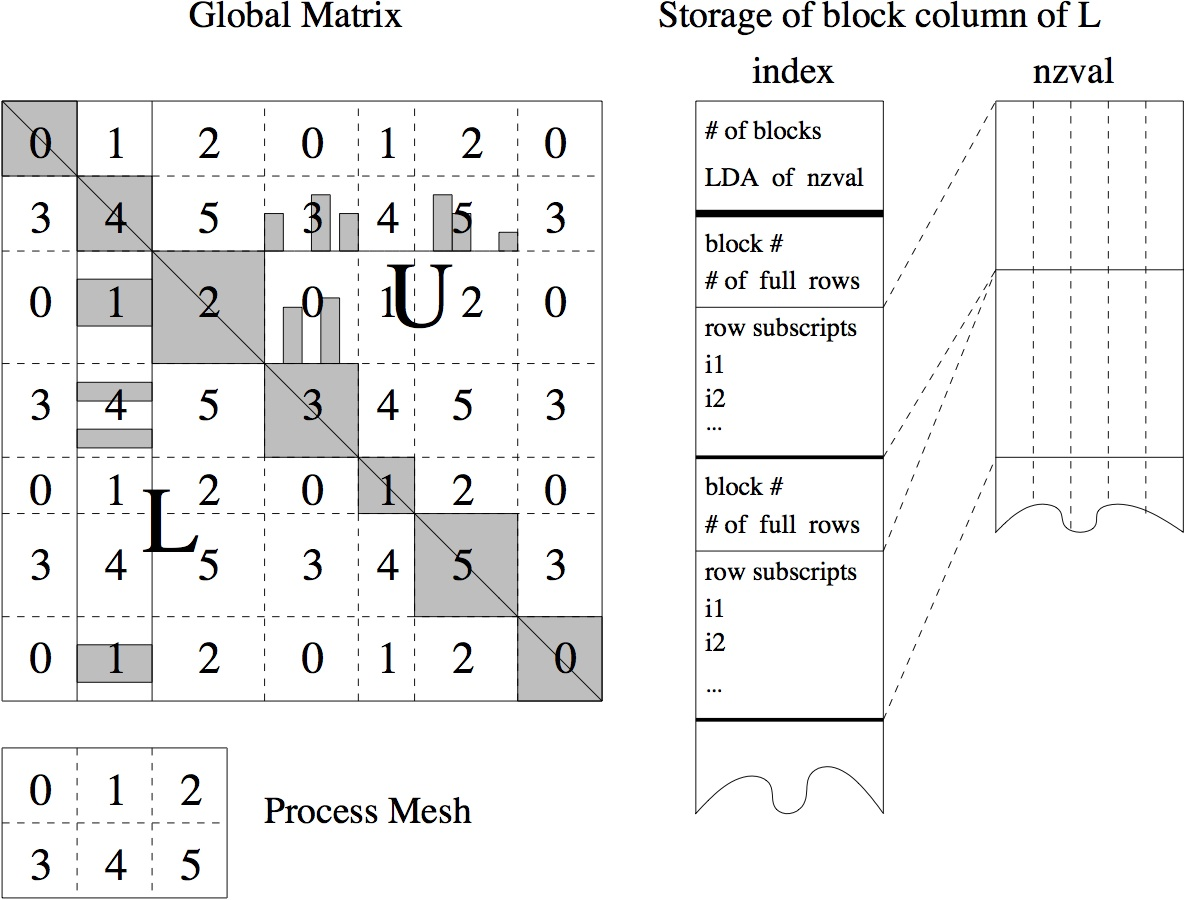
\includegraphics[width=0.6\textwidth]{lu_2d.jpg} }%
%\vspace{-5mm}
\caption{The 2 block-cyclic layout and the data structure
	to store a local block column of $L$.}
\label{fig:lu_2d}
\end{figure}


\section{Process grid and MPI communicator}
\label{sec:grid}
All MPI applications begin with a default communication domain
that includes all processes, say $N_p$, of this parallel job.
The default communicator {\tt MPI\_COMM\_WORLD} represents
this communication domain.
The $N_p$ processes are identified as a linear array of process IDs in the
range $0\;\ldots\;N_p-1$.

\subsection{2D process grid}
For {\superlud} library, we create a new process group derived from an
existing group using $N_g$ processes. There is a good
reason to use a new group rather than {\tt MPI\_COMM\_WORLD}, that is,
the message passing calls of the SuperLU library will be isolated
from those in other libraries or in the user's code.
For better scalability of the $LU$ factorization, we map the
1D array of $N_g$ processes into a logical 2D process grid.
This grid will have {\tt nprow} process rows and {\tt npcol} process columns,
such that ${\tt nprow} * {\tt npcol} = N_g$. A process can be referenced
either by its rank in the new group or by its coordinates within
the grid.
The routine {\tt superlu\_gridinit} maps already-existing processes
to a 2D process grid.
% A typical code fragment to accomplish this task would be the following:

\begin{verbatim}
    superlu_gridinit(MPI_Comm Bcomm, int nprow, int npcol, gridinfo_t *grid);
\end{verbatim}

%{\em Note that the underlined arguments in the calling sequence
%denote output arguments.}
This process grid will use the first ${\tt nprow} * {\tt npcol}$
processes from the base MPI communicator {\tt Bcomm}, and assign them
to the grid in a row-major ordering.
The input argument {\tt Bcomm} is an MPI communicator
representing the existing base group upon which the new
group will be formed. For example, it can be
{\tt MPI\_COMM\_WORLD}. The output argument {\tt grid}
represents the derived group to be used in {\superlud}.
{\tt Grid} is a structure containing the following fields:
\begin{verbatim}
   struct {
       MPI_Comm comm;        /* MPI communicator for this group */
       int iam;              /* my process rank in this group   */
       int nprow;            /* number of process rows          */
       int npcol;            /* number of process columns       */
       superlu_scope_t rscp; /* process row scope               */
       superlu_scope_t cscp; /* process column scope            */
   } grid;
\end{verbatim}

In the $LU$ factorization, some communications occur only among
the processes in a row (column), not among all processes.
For this purpose, we introduce two process subgroups,
namely {\tt rscp} (row scope) and {\tt cscp} (column scope).
For {\tt rscp} ({\tt cscp}) subgroup,
all processes in a row (column) participate in the communication.

The macros {\tt MYROW(iam, grid)} and {\tt MYCOL(iam, grid)} give
the row and column coordinates in the 2D grid of the process 
who has rank {\tt iam}.

\paragraph\
{\em NOTE: All processes in the base group, including those not in the
new group, must call this grid creation routine. This is required by
the MPI routine {\tt MPI\_Comm\_create} to create a new communicator.}


\subsection{Arbitrary grouping of processes}
It is sometimes desirable to divide up the processes into several subgroups,
each of which performs independent work of a single application.
In this situation, we cannot simply use the first ${\tt nprow} * {\tt npcol}$
processes to define the grid.
A more sophisticated process-to-grid mapping routine
{\tt superlu\_gridmap} is designed to create a grid with
processes of arbitrary ranks.
% A typical code fragment would be the following:

\begin{verbatim}
    superlu_gridmap(MPI_Comm Bcomm, int nprow, int npcol,
                    int usermap[], int ldumap, gridinfo_t *grid);
\end{verbatim}

The array {\tt usermap[]} contains the processes to be used
in the newly created grid. {\tt usermap[]} is indexed like a
Fortran-style 2D array with {\tt ldumap} as the leading dimension.
So {\tt usermap[i+j$*$ldumap]} (i.e., {\tt usermap(i,j)} in
Fortran notation) holds the process rank
to be placed in \{i, j\} position of the 2D process grid.
After grid creation, this subset of processes is logically numbered
in a consistent manner with the initial set of processes; that is,
they have the ranks in the range $0\;\ldots\;{\tt nprow} * {\tt npcol}-1$
in the new grid.
For example, if we want to map 6 processes with ranks $11\;\ldots\;16$
into a $2\times 3$ grid, we define
${\tt usermap} = \{11, 14, 12, 15, 13, 16\}$ and ${\tt ldumap}=2$.
Such a mapping is shown below
\begin{center}
\begin{tabular}{c|c|c|c|}
\multicolumn{1}{c}{} &\multicolumn{1}{c}{0}
  &\multicolumn{1}{c}{1}
  &\multicolumn{1}{c}{2}\\\cline{2-4}
0 &11 &12 &13 \\\cline{2-4}
1 &14 &15 &16 \\\cline{2-4}
\end{tabular}
\end{center}

\paragraph\
{\em NOTE: All processes in the base group, including those not in
the new group, must call this routine.}

{\tt Superlu\_gridinit} simply calls {\tt superlu\_gridmap}
with {\tt usermap[]} holding the first ${\tt nprow} * {\tt npcol}$
process ranks.

%%%%%%%%%%%%%%%%%%%%%%%%%%%%%%%%%%%%%%%%%%%%%%%%%%%%%%%%%%%%%%%%%%%%%%%
\section{Algorithmic background}
Although partial pivoting is used in both sequential and shared-memory
parallel factorization algorithms, it is not used in the
distributed-memory parallel algorithm, because it requires dynamic adaptation
of data structures and load balancing, and so is hard to make it scalable.
We use alternative techniques to stabilize the algorithm, which include
statically pivot large elements to the diagonal, single-precision
diagonal adjustment to avoid small pivots, and iterative refinement.
Figure~\ref{fig:GESP_alg} sketches our GESP algorithm
(Gaussian elimination with Static Pivoting).
Numerical experiments show that for a wide range of problems,
GESP is as stable as GEPP~\cite{lidemmel03}.

\begin{figure}[htbp]
\begin{tabbing}
jnk \= jnk \= jnk \= jnk \= jnk \= jnk \= xxxxx \= xxxxxxxxxxxxxxx \kill
\>(1) Perform row/column equilibration and row permutation:
	$A \leftarrow P_r\cdot D_r\cdot A\cdot D_c$, \\
\> \>	where $D_r$ and $D_c$ are diagonal matrices and $P_r$ is a row 
        permutation chosen \\
\> \>	to make the diagonal large compared to the off-diagonal.\\
\>(2) Find a column permutation $P_c$ to preserve sparsity:
	$A\leftarrow P_c\cdot A\cdot P_c^T$ \\
\>(3) Perform symbolic analysis to determine the nonzero structures of $L$ and $U$.\\
\>(4) Factorize $A=L\cdot U$ with control of diagonal magnitude: \\
\>\>\> {\bf if} ( $|a_{ii}| < \sqrt{\varepsilon}\cdot \|A\|_1$ ) {\bf then} \\
\>\>\>\> set $a_{ii}$ to $\sqrt{\varepsilon}\cdot \|A\|_1$\\
\>\>\> {\bf endif} \\
\>(5) Perform triangular solutions using $L$ and $U$.\\
\>(6) If needed, use an iterative solver like GMRES or iterative refinement (shown below) \\
\>\>\>{\bf iterate}:\\
\>\>\>\>$r = b - A\cdot x$  \hspace{0.98in} $\ldots$ sparse matrix-vector 
multiply \\
\>\>\>\>Solve $A\cdot dx = r$     \hspace{.77in} $\ldots$ triangular solution\\
\>\>\>\>$berr = \max_i\frac{|r|_i}{(|A|\cdot|x|+|b|)_i}$
                    \hspace{.3in} $\ldots$ componentwise backward error \\
\>\>\>\>{\bf if} ( $berr > \varepsilon$ and 
		   $berr \le \frac{1}{2}\cdot lastberr$ )
%\>\>\>\>{\bf if} ( $\frac{\|dx\|}{\|x\|} > \varepsilon$ 
%		   and $\frac{\|r\|}{\|A\|_1\cdot\|x\|} > \varepsilon$ )
%		   and $\|dx\| < last\_d$ )
	{\bf then} \\
\>\>\>\>\> $x = x + dx$   \\
\>\>\>\>\> $lastberr = berr$\\
\>\>\>\>\>{\bf goto iterate} \\
\>\>\>\>{\bf endif} \\
\>(7) If desired, estimate the condition number of $A$
\end{tabbing}
\caption{The outline of the GESP algorithm.}
\label{fig:GESP_alg}
\end{figure}

\ignore{ %%%%%%%%%%%%%%%%%%%%
\begin{figure}
\begin{tabbing}
jnk \= jnk \= jnk \= jnk \= jnk \= jnk \= xxxxx \= xxxxxxxxxxxxxxx \kill
\>(1) Row/column equilibration: $A \leftarrow D_r\cdot A\cdot D_c$ \\
\> \>	$D_r$ and $D_c$ are diagonal matrices chosen so that the
	largest entry of each row and \\
\> \>   column is $\pm 1$. \\
\>(2) Row permutation:  $A \leftarrow P_r \cdot A$ \\
\> \>	$P_r$ is a row permutation chosen to make the diagonal large
	compared to the off-diagonal.\\
% \>(2) Find a row permutation $P_r$ to put large entries on the diagonal:
% 	 $A\leftarrow P_r\cdot  A$ \\
%\>\>\>{\bf if} ( there are zeros on diagonal of $A$ ) {\bf then} \\
%\>\>\>\>1) drop $a_{ij}$ if $|a_{ij}| < \eta\cdot ||A||$
%	\ \ ( $\eta = 10^{-7}, 10^{-5}, ..., 10^{-1}$ ) \\
%\>\>\>\>2) apply maximum bipartite matching to the new $A$ \\
%\>\>\>{\bf endif} \\
\>(3) Find a column permutation $P_c$ to preserve sparsity:
	$A\leftarrow P_c\cdot A\cdot P_c^T$ \\
\>(4) Factorize $A=L\cdot U$ with control of diagonal magnitude \\
\>\>\> {\bf if} ( $|a_{ii}| < \sqrt{\varepsilon}\cdot ||A||$ ) {\bf then} \\
\>\>\>\> set $a_{ii}$ to $\sqrt{\varepsilon}\cdot ||A||$\\
\>\>\> {\bf endif} \\
\>(5) Solve $A\cdot x=b$ using the $L$ and $U$ factors, with the following
	iterative refinement \\
\>\>\>{\bf iterate}:\\
\>\>\>\>$r = b - A\cdot x$  \hspace{1in} $\ldots$ sparse matrix-vector 
multiply \\
\>\>\>\>Solve $A\cdot dx = r$     \hspace{.78in} $\ldots$ triangular solution\\
\>\>\>\>$berr = \max_i\frac{|r|_i}{(|A|\cdot|x|+|b|)_i}$
                    \hspace{.3in} $\ldots$ componentwise backward error \\
\>\>\>\>{\bf if} ( $berr > \varepsilon$ and 
		   $berr \le \frac{1}{2}\cdot lastberr$ )
%\>\>\>\>{\bf if} ( $\frac{||dx||}{||x||} > \varepsilon$ 
%		   and $\frac{||r||}{||A||\cdot||x||} > \varepsilon$ )
%		   and $||dx|| < last\_d$ )
	{\bf then} \\
\>\>\>\>\>$x = x + dx$   \\
 \>\>\>\>\>$lastberr = berr$\\
\>\>\>\>\>{\bf goto iterate} \\
\>\>\>\>{\bf endif} \\
\end{tabbing}
\vspace*{-.3in}
\caption{The outline of the GESP algorithm.}
\label{fig:GESP_alg}
\end{figure}
} %%%% ignore

Step (1) is accomplished by a weighted bipartite matching algorithm
due to Duff and Koster~\cite{duffkoster99}. Currently, process 0
computes $P_r$ and then broadcasts it to all the other processes.
If the distributed input interface is used (Section~\ref{sec:DistInput}),
we first gather the distributed matrix $A$  onto processor 0.
Work is underway to remove this sequential bottleneck.

In Step (2), we provide several ordering options, such as 
multiple minimum degree ordering~\cite{liu85} on the graphs of 
$A+A^T$, or the {\metis}~\cite{kaku:98a} ordering on the graphs of $A+A^T$.
% and the approximate minimum degree column ordering~\cite{davisgilbert00}.
The user can use any other ordering in place of the ones provided
in the library.
({\em Note, since we will pivot on the diagonal in step (4),
an ordering based on the structure of $A+A^T$ almost always yields sparser
factors than that based on the structure of $A^TA$.
This is different from SuperLU and SuperLU\_MT, where we allow to pivot
off-diagonal.})
In this step, when a sequential ordering algorithm is used, every process
runs the same algorithm independently.

Step (3) can be done either sequentially or in parallel
depending on how the \textsf{options} argument is set
(see Section~\ref{sec:drivers} for details.)
The parallel symbolic factorization was a newly added feature
since the \textsf{v2.1} release. 
It is designed tightly around the separator tree returned from
a graph partitioning type of ordering (presently we use
{\parmetis}~\cite{kaku:03}), and works only on power-of-two
processors.  We first re-distribute the graph of $A$
onto the largest $2^q$ number of processors
which is smaller than the total $N_p$ processors, then perform
parallel symbolic factorization, and finally re-populate the
$\{L \backslash U\}$ structure to all $N_p$ processors.
The algorithm and performance was studied in~\cite{grigoridemmelli07}.
To invoke parallel symbolic factorization, the user needs to set
the two fields of the \textsf{options} argument as follows:
\begin{verbatim}
    options.ParSymbFact       = YES
    options.ColPerm           = PARMETIS;
\end{verbatim}
Note that, even if the user sets \textsf{options.ColPerm} to use an ordering
algorithm other than {\parmetis}, the driver routine overrides it with
{\parmetis} when it sees \textsf{options.ParSymbFact = YES}.

Steps (4) to (7) are the most time-consuming steps and were parallelized
a while ago, see the papers~\cite{lidemmel03,li05}.


\subsection{Multicore and GPU enhancements}
Given that the node architecture trend is to have many simpler cores
on a NUMA node, possibly with GPU-like accelerators, and the
amount of memory per-core becomes smaller, the pure MPI model
does not match the light-weight processor architecture.
We need to resort to other forms of parallelism
at node level. In sparse factorization (step (4) in Figure~\ref{fig:GESP_alg}),
the Schur complement update after each panel factorization step exhibits
ample fine-grid parallelism. We have designed the OpenMP + CUDA
code to exploit the on-node parallelism. For each MPI task of the 
Schur complement update, we aggegrate the small $L$ and $U$ matrix blocks
into a larger block, divide the GEMM work between CPU and GPU using
some heuristic performance model, offload the larger block of GEMM
to GPU.  The key to success is to overlap the CPU work 
(multithreaded Scatter/Gather, some portion of GEMM) with
the GPU work (GEMM with multiple CUDA streams). This way, we are able
to hide the latency time due to PCI bus transfer between CPU and GPU.
The detailed algorithm description and performance data were given
in the paper by Sao et al.~\cite{sao2014}.

To use Nvidia GPU, you must set the following
Linux shell environment variable before compilation:

\vspace{.1in}
{\tt setenv ACC GPU}
\vspace{.1in}

Hybrid MPI+OpenMP setting may outperform MPI-only configurations in some
cases and in most cases hybrid MPI+OpenMP would require less memory.
The environment variable {\tt OMP\_NUM\_THREADS} needs to be set appropriately.
Hybrid configuration obtains threaded parallelism from both,
explicit OpenMP pragmas and multithreaded BLAS. Thus for good performance
it is better if OpenMP threading library and BLAS threading are synergistic.
For example, when using Intel MKL libray, just setting {\tt OMP\_NUM\_THREADS}
would set the number of threads for both MKL and OpenMP. However,
it is possible to have different number of threads for MKL, in which case
{\tt MKL\_NUM\_THREADS} controls the number of threads used by MKL. 
In our case, just setting {\tt OMP\_NUM\_THREADS} is sufficient. 

Triangular solve phase does not use multithreading yet.
The MPI-only configuration may be more suitable in case of
many right hand sides or in other cases, where solve phase seems
to be a performance bottleneck.


\section{{\tt Options} argument}
\label{sec:options}
One important input argument is {\tt options}, which controls how the
linear system will be solved.
Although the algorithm presented in~\fig{GESP_alg} consists of
seven steps, for some matrices not all steps are needed to get
accurate solution. For example, for diagonally dominant matrices, 
choosing the diagonal pivots ensures the stability;
there is no need for row pivoting in step (1).
In another situation where a sequence of matrices with the
same sparsity pattern need be factorized, the column
permutation $P_c$ (and also the row permutation $P_r$, if
the numerical values are similar) need be computed only
once, and reused thereafter. ($P_r$ and $P_c$
are implemented as permutation vectors {\tt perm\_r} and {\tt perm\_c}.)
For the above examples, performing all seven steps does more
work than necessary. 
{\tt Options} is used to accommodate the various requirements of applications;
it contains the following fields:
\begin{itemize}
\item {\tt Fact}\\
    Specifies whether or not the factored form of the matrix
    $A$ is supplied on entry, and if not, how the matrix $A$ will
    be factored base on some assumptions of the previous history.
    {\tt fact} can be one of:
    \begin{itemize}
    \item {\tt DOFACT}: the matrix $A$ will be factorized from scratch.
    \item {\tt SamePattern}: the matrix $A$ will be factorized assuming
	that a factorization of a matrix with the same sparsity pattern
	was performed prior to this one. Therefore, this factorization
        will reuse column permutation vector {\tt perm\_c}.
    \item {\tt SampPattern\_SameRowPerm}: the matrix $A$ will be factorized
	assuming that a factorization of a matrix with the same sparsity
	pattern and similar numerical values was performed prior to this one.
        Therefore, this factorization will reuse both row and column
        permutation vectors {\tt perm\_r} and {\tt perm\_c}, both row and
	column scaling factors $D_r$ and $D_c$, and the distributed data
	structure set up from the previous symbolic factorization.
    \item {\tt FACTORED}: the factored form of $A$ is input.
    \end{itemize}
\item {\tt Equil}  \{ {\tt YES} $|$ {\tt NO} \} \\
    Specifies whether to equilibrate the system.
\item {\tt ParSymbFact}   \{ {\tt YES} $|$ {\tt NO} \} \\ 
    Specifies whether to perform parallel symbolic factorization.
    If it is set to \textsf{YES}, the \textsf{ColPerm} field should
    be set to \textsf{PARMETIS}. Otherwise, the driver routine {\tt pdgssvx}
    will use {\parmetis} anyway, ignoring the other setting in
    \textsf{ColPerm}.
\item {\tt ColPerm}\\
    Specifies the column ordering method for fill reduction.
    \begin{itemize}
    \item {\tt NATURAL}: natural ordering.
    \item {\tt MMD\_AT\_PLUS\_A}: minimum degree ordering on the
			structure of $A^T+A$.
    \item {\tt MMD\_ATA}: minimum degree ordering on the structure of
			$A^TA$.
    \item {\tt METIS\_AT\_PLUS\_A}: {\metis} ordering on the
			structure of $A^T+A$.
    \item {\tt PARMETIS}: {\parmetis} ordering on the structure of $A^T+A$.
%            This can only be used with parallel symbolic factorization
%            (i.e., {\tt ParSymbFact = YES}).
    \item {\tt MY\_PERMC}: use the ordering given in {\tt perm\_c} input by
	                the user.
    \end{itemize}
\item {\tt RowPerm} \\
    Specifies how to permute rows of the original matrix.
    \begin{itemize}
    \item {\tt NATURAL}: use the natural ordering.
    \item {\tt LargeDiag\_MC64}: use a serial, weighted bipartite matching
      algorithm implemented in MC64 to permute the rows to make the
      diagonal large relative to the off-diagonal~\cite{duffkoster01}.
    \item {\tt LargeDiag\_AWPM}: use a parallel, approximate weighted bipartite
      matching algorithm implemented in CombBLAS to permute the rows to
      make the diagonal large relative to the off-diagonal~\cite{awpm}.
    \item {\tt MY\_PERMR}: use the ordering given in {\tt perm\_r} input by the user.
    \end{itemize}
\item {\tt ReplaceTinyPivot} \{ {\tt YES} $|$ {\tt NO} \} \\ 
    Specifies whether to replace the tiny diagonals by
           $\sqrt\varepsilon\cdot||A||$ during $LU$ factorization.
\item {\tt IterRefine}\\
    Specifies how to perform iterative refinement.
    \begin{itemize}
    \item {\tt NO}: no iterative refinement.
    \item {\tt DOUBLE}: accumulate residual in double precision.
    \item {\tt EXTRA}:  accumulate residual in extra precision.
	 ({\em not yet implemented.})
    \end{itemize}
\item {\tt Trans}  \{ {\tt NOTRANS} $|$ {\tt TRANS} $|$ {\tt CONJ} \} \\
    Specifies whether to solve the transposed system.
\item {\tt SolveInitialized}  \{ {\tt YES} $|$ {\tt NO} \} \\
    Specifies whether the initialization has been performed to
    the triangular solve. \\
   (used only by the distributed input interface)
\item {\tt RefineInitialized}  \{ {\tt YES} $|$ {\tt NO} \} \\
    Specifies whether the initialization has been performed to
    the sparse matrix-vector multiplication routine needed in the
    iterative refinement. \\
    (used only by the distributed input interface)
\item {\tt num\_lookaheads}  \{ integer \} \\
    Specifies the number of levels in the look-ahead factorization
\item {\tt lookahead\_etree}  \{ {\tt YES} $|$ {\tt NO} \} \\
    Specifies whether to use the elimination tree computed from the 
    serial symbolic factorization to perform static scheduling.
\item {\tt SymPattern}  \{ {\tt YES} $|$ {\tt NO} \} \\
    Gives the scheduling algorithm a hint whether the matrix
    has the symmetric pattern.
 \item {\tt PrintStat}  \{ {\tt YES} $|$ {\tt NO} \} \\
    Specifies whether to print the solver's statistics.
\end{itemize}

There is a routine named {\tt set\_default\_options\_dist()} that sets the
default values of these options, which are:
\begin{verbatim}
    fact              = DOFACT           /* factor from scratch */
    equil             = YES
    ParSymbFact       = NO
    colperm           = MMD_AT_PLUS_A
    rowperm           = LargeDiag        /* use MC64 */
    ReplaceTinyPivot  = YES
    IterRefine        = DOUBLE
    Trans             = NOTRANS
    SolveInitialized  = NO
    RefineInitialized = NO
    num_lookaheads    = 10;
    lookahead_etree   = NO;
    SymPattern        = NO;
    PrintStat         = YES
\end{verbatim}


\section{Basic steps to solve a linear system}
In this section, we use a complete sample program to illustrate
the basic steps required to use {\superlud}.
This program is listed below, and is also available
as {\tt EXAMPLE/pddrive.c} in the source code distribution.
All the routines must include the header file {\tt superlu\_ddefs.h}
(or {\tt superlu\_zdefs.h}, the complex counterpart)
which contains the definitions of the data types, the macros and
the function prototypes.

\begin{verbatim}
#include <math.h>
#include "superlu_ddefs.h"

main(int argc, char *argv[])
/*
 * Purpose
 * =======
 *
 * The driver program PDDRIVE.
 *
 * This example illustrates how to use PDGSSVX with the full
 * (default) options to solve a linear system.
 * 
 * Five basic steps are required:
 *   1. Initialize the MPI environment and the SuperLU process grid
 *   2. Set up the input matrix and the right-hand side
 *   3. Set the options argument
 *   4. Call pdgssvx
 *   5. Release the process grid and terminate the MPI environment
 *
 * On the Cray T3E, the program may be run by typing
 *    mpprun -n <procs> pddrive -r <proc rows> -c <proc columns> <input_file>
 *
 */
{
    superlu_options_t options;
    SuperLUStat_t stat;
    SuperMatrix A;
    ScalePermstruct_t ScalePermstruct;
    LUstruct_t LUstruct;
    SOLVEstruct_t SOLVEstruct;
    gridinfo_t grid;
    double   *berr;
    double   *b, *xtrue;
    int_t    m, n, nnz;
    int_t    nprow, npcol;
    int      iam, info, ldb, ldx, nrhs;
    char     trans[1];
    char     **cpp, c;
    FILE *fp, *fopen();

    nprow = 1;  /* Default process rows.      */
    npcol = 1;  /* Default process columns.   */
    nrhs = 1;   /* Number of right-hand side. */

    /* ------------------------------------------------------------
       INITIALIZE MPI ENVIRONMENT. 
       ------------------------------------------------------------*/
    MPI_Init( &argc, &argv );

    /* Parse command line argv[]. */
    for (cpp = argv+1; *cpp; ++cpp) {
        if ( **cpp == '-' ) {
            c = *(*cpp+1);
            ++cpp;
            switch (c) {
              case 'h':
                  printf("Options:\n");
                  printf("\t-r <int>: process rows    (default %d)\n", nprow);
                  printf("\t-c <int>: process columns (default %d)\n", npcol);
                  exit(0);
                  break;
              case 'r': nprow = atoi(*cpp);
                  break;
              case 'c': npcol = atoi(*cpp);
                  break;
            }
        } else { /* Last arg is considered a filename */
            if ( !(fp = fopen(*cpp, "r")) ) {
                ABORT("File does not exist");
            }
            break;
        }
    }

    /* ------------------------------------------------------------
       INITIALIZE THE SUPERLU PROCESS GRID. 
       ------------------------------------------------------------*/
    superlu_gridinit(MPI_COMM_WORLD, nprow, npcol, &grid);

    /* Bail out if I do not belong in the grid. */
    iam = grid.iam;
    if ( iam >= nprow * npcol )	goto out;

    /* ------------------------------------------------------------
       GET THE MATRIX FROM FILE AND SETUP THE RIGHT HAND SIDE. 
       ------------------------------------------------------------*/
    dcreate_matrix(&A, nrhs, &b, &ldb, &xtrue, &ldx, fp, &grid);

    if ( !(berr = doubleMalloc_dist(nrhs)) )
        ABORT("Malloc fails for berr[].");

    /* ------------------------------------------------------------
       NOW WE SOLVE THE LINEAR SYSTEM.
       ------------------------------------------------------------*/

    /* Set the default input options. */
    set_default_options_dist(&options);

    m = A.nrow;
    n = A.ncol;

    /* Initialize ScalePermstruct and LUstruct. */
    ScalePermstructInit(m, n, &ScalePermstruct);
    LUstructInit(n, &LUstruct);

    /* Initialize the statistics variables. */
    PStatInit(&stat);

    /* Call the linear equation solver. */
    pdgssvx(&options, &A, &ScalePermstruct, b, ldb, nrhs, &grid,
            &LUstruct, &SOLVEstruct, berr, &stat, &info);


    /* Check the accuracy of the solution. */
    pdinf_norm_error(iam, ((NRformat_loc *)A.Store)->m_loc,
                     nrhs, b, ldb, xtrue, ldx, &grid);

    PStatPrint(&options, &stat, &grid);        /* Print the statistics. */

    /* ------------------------------------------------------------
       DEALLOCATE STORAGE.
       ------------------------------------------------------------*/

    PStatFree(&stat);
    Destroy_CompRowLoc_Matrix_dist(&A);
    ScalePermstructFree(&ScalePermstruct);
    Destroy_LU(n, &grid, &LUstruct);
    LUstructFree(&LUstruct);
    if ( options.SolveInitialized ) {
        dSolveFinalize(&options, &SOLVEstruct);
    }
    SUPERLU_FREE(b);
    SUPERLU_FREE(xtrue);
    SUPERLU_FREE(berr);

    /* ------------------------------------------------------------
       RELEASE THE SUPERLU PROCESS GRID.
       ------------------------------------------------------------*/
out:
    superlu_gridexit(&grid);

    /* ------------------------------------------------------------
       TERMINATES THE MPI EXECUTION ENVIRONMENT.
       ------------------------------------------------------------*/
    MPI_Finalize();

}
\end{verbatim}

Five basic steps are required to call a SuperLU routine:
\begin{enumerate}
\item Initialize the MPI environment and the SuperLU process grid.\\
	This is achieved by the calls to the MPI routine {\tt MPI\_Init()}
	and the SuperLU routine\\ {\tt superlu\_gridinit()}.
	In this example, the communication domain for SuperLU is built upon
	the MPI default communicator {\tt MPI\_COMM\_WORLD}.
	In general, it can be built upon any MPI communicator.
	\Cref{sec:grid} contains the details about this step.
\item Set up the input matrix and the right-hand side.\\
        This example uses the interface with the distributed input matrices,
        see Section~\ref{sec:DistInput}.
        In most practical applications, the matrices can be
        generated on each process without the need to have a centralized
        place to hold them.
        But for this example, we let process 0 read the input matrix stored
        on disk	in Harwell-Boeing format~\cite{duffgrimes92}
        (a.k.a. compressed column storage), and distribute it to all the
        other processes, so that each process only owns a block of rows of
        matrix. The right-hand side matrix is generated
	so that the exact solution matrix consists of all ones.
        The subroutine {\tt dcreate\_matrix()} accomplishes this task.
\item Initialize the input arguments: {\tt options, ScalePermstruct, LUstruct,
        stat}.\\
        The input argument {\tt options} controls how the linear system would
  	be solved---use equilibration or not, how to order the rows and
	the columns of the matrix, use iterative refinement or not.
	The subroutine {\tt set\_default\_options\_dist()} sets the
        {\tt options} argument so that the solver performs all the
        functionality. You can also set it up according to your own needs,
        see section~\ref{sec:options} for the fields of this structure.
        {\tt ScalePermstruct} is the data structure that stores 
	the several vectors describing the transformations
        done to $A$. {\tt LUstruct} is the data structure
        in which the distributed $L$ and $U$ factors are stored.
	{\tt Stat} is a structure collecting the statistics about
	runtime and flop count, etc.
\item Call the SuperLU routine {\tt pdgssvx()}.
\item Release the process grid and terminate the MPI environment.\\
	After the computation on a process grid has been completed, the
	process grid should be released by a call to the SuperLU routine
	{\tt superlu\_gridexit()}.
        When all computations have been completed, the MPI routine
        {\tt MPI\_Finalize()} should be called.
\end{enumerate}


\section{User-callable routines}
%% Appendix~\ref{chap:superlu_dist_spec} contains the complete specifications
%% of the routines in SuperLU\_DIST.

\subsection{Driver routines}
\label{sec:drivers}
There are two driver routines to solve systems of linear equations,
which are named {\tt pdgssvx\_ABglobal} for the global input interface,
and {\tt pdgssvx} for the distributed interface.
We recommend that the general users, especially the beginners, 
use a driver routine rather than the computational
routines, because correctly using the driver routine does not require
thorough understanding of the underlying data structures.
Although the interface of these routines are simple, we expect their rich 
functionality can meet the requirements of most applications.
{\tt Pdgssvx\_ABglobal}/{\tt pdgssvx} perform the following functions:
\begin{itemize}
\item Equilibrate the system (scale $A$'s rows and columns to
	have unit norm) if $A$ is poorly scaled;
\item Find a row permutation that makes diagonal of $A$ large
	relative to the off-diagonal;
\item Find a column permutation that preserves the sparsity of
	the $L$ and $U$ factors;
\item Solve the system $AX=B$ for $X$ by factoring $A$
	followed by forward and back substitutions;
\item Refine the solution $X$.
\end{itemize}


\subsection{Computational routines}
The experienced users can invoke the following computational routines
to directly control the behavior of {\superlud} in order to meet their
requirements.
\begin{itemize}
\item {\tt pdgstrf()}: Factorize in parallel. \\
	This routine factorizes the input matrix $A$ (or the scaled and
	permuted $A$). It assumes that the distributed data structures
	for $L$ and $U$ factors are already set up, and the initial
  	values of $A$ are loaded into the data structures.
	If not, the routine {\tt symbfact()} should be called to
	determine the nonzero patterns of the factors, and the
	routine {\tt pddistribute()} should be called to distribute the matrix.
	{\tt Pdgstrf()} can factor non-square matrices.
%	Currently, $A$ must be globally available on all processes.
\item {\tt pdgstrs()/pdgstrs\_Bglobal()}: Triangular solve in parallel. \\
	This routine solves the system by forward and back
	substitutions using the the $L$ and $U$ factors
	computed by {\tt pdgstrf()}. {\tt Pdgstrs()} takes distributed $B$.
	For {\tt pdgstrs\_Bglobal()}, $B$ must be globally available on
        all processes. 
\item {\tt pdgsrfs()/pdgsrfs\_ABXglobal()}: Refine solution in parallel. \\
	Given $A$, its factors $L$ and $U$, and an initial solution
	$X$, this routine performs iterative refinement.
	{\tt Pdgsrfs()} takes distributed $A$, $B$ and $X$.
	For {\tt pdgsrfs\_ABXglobal()}, $A$, $B$ and $X$ must be globally
        available on all processes. 
\end{itemize}

\subsection{Utility routines}
\label{sec:slud_utility}

The following utility routines can help users create and destroy the
{\superlud} matrices. These routines reside in three places: {\tt SRC/util.c},
{\tt SRC/\{d,z\}util.c}, and {\tt SRC/p\{d,z\}util.c}.
Most of the utility routines in sequential {\superlu} can also be used
in {\superlud} for the local data, see Section~\ref{sec:slu_utility}.
Here, we only list those new routines
specific to {\superlud}. Note that in order to avoid name clash between
{\superlu} and {\superlud}, we append ``{\tt \_dist}'' to each routine
name in {\superlud}.

\begin{verbatim}
    /* Create a supermatrix in distributed compressed row format. A is output. */
    dCreate_CompRowLoc_Matrix_dist(SuperMatrix *A, int_t m, int_t n,
                                   int_t nnz_loc, int_t m_loc, int_t fst_row,
                                   double *nzval, int_t *colind, int_t *rowptr,
                                   Stype_t stype, Dtype_t dtype, Mtype_t mtype);

    /* Deallocate the supermatrix in distributed compressed row format. */
    Destroy_CompRowLoc_Matrix_dist(SuperMatrix *A);

    /* Allocate storage in ScalePermstruct. */
    ScalePermstructInit(const int_t m, const int_t n,
                        ScalePermstruct_t *ScalePermstruct);

    /* Deallocate ScalePermstruct */
    ScalePermstructFree(ScalePermstruct_t *ScalePermstruct);

    /* Allocate storage in LUstruct. */
    LUstructInit(const int_t n, LUstruct_t *LUstruct);

    /* Deallocate the distributed L & U factors in LUstruct. */
    Destroy_LU(int_t n, gridinfo_t *grid, LUstruct_t *LUstruct);

    /* Deallocate LUstruct. */
    LUstructFree(LUstruct_t *LUstruct);

    /* Initialize the statistics variable. */
    PStatInit(SuperLUStat_t *stat);

    /* Print the statistics. */
    PStatPrint(superlu_options_t *options, SuperLUStat_t *stat,
               gridinfo_t *grid);

    /* Deallocate the statistics variable. */
    PStatFree(SuperLUStat_t *stat);
\end{verbatim}


\section{Installation}
\label{sec:dist_install}
\subsection{File structure and complilation}
The top level SuperLU\_DIST/ directory is structured as follows:
\begin{verbatim}
    SuperLU_DIST/README.md instructions on installation
    SuperLU_DIST/CBLAS/    BLAS routines in C, functional but not fast
    SuperLU_DIST/DOC/      Users' Guide
    SuperLU_DIST/EXAMPLE/  example programs
    SuperLU_DIST/INSTALL/  test machine dependent parameters
    SuperLU_DIST/SRC/      C source code, to be compiled into libsuperlu_dist.a
    SuperLU_DIST/lib/      contains library archive libsuperlu_dist.a
    SuperLU_DIST/Makefile  top level Makefile that does installation and testing
    SuperLU_DIST/make.inc  compiler, compiler flags, library definitions and C
                           preprocessor definitions, included in all Makefiles.
                           (You may need to edit it to suit for your system
                            before compiling the whole package.)
    SuperLU_DIST/MAKE_INC/ sample machine-specific make.inc files
\end{verbatim}

You can use CMake automic build system to install the package. Please see
README.md for instruction. The following describes how to install manually
by editing a Makefile.

Before installing the package, you may need to edit
{\tt SuperLU\_DIST/make.inc} for your system.
This make include file is referenced inside all the Makefiles
in the various subdirectories. As a result, there is no need to 
edit the Makefiles in the subdirectories. All information that is
machine specific has been defined in this include file. 

Sample machine-specific {\tt make.inc} are provided in the
{\tt MAKE\_INC/} directory for several platforms, such as
Cray XE6 and IBM SP.
When you have selected the machine to which you wish to install
{\superlud}, you may copy the appropriate sample include file
(if one is present) into {\tt make.inc}. For example, if you wish to run
on a Cray XE6,  you can do:

\hspace{.4in}{\tt cp MAKE\_INC/make.xe6 make.inc}

For the systems other than those listed above, slight modifications to the
{\tt make.inc} file will need to be made.
In particular, the following items should be examined:
\begin{enumerate}   
\item The BLAS library.\\
   If there is a BLAS library available on your machine,
   you may define the following in {\tt make.inc}:

   \hspace{.4in}{\tt BLASDEF = -DUSE\_VENDOR\_BLAS}

   \vspace{-6pt}
   \hspace{.4in}{\tt BLASLIB = <BLAS library you wish to link with>}

   The {\tt CBLAS/} subdirectory contains the part of the BLAS (in C) needed by
   {\tt SuperLU\_DIST} package. However, these routines are intended for use
   only if there is no faster implementation of the BLAS already available
   on your machine. In this case, you should do the following:
   \begin{itemize}
   \item[1)]In make.inc, undefine (comment out) BLASDEF, define:

          \hspace{.4in}{\tt BLASLIB = ../lib/libblas\$(PLAT).a}

   \item[2)] At the top level SuperLU\_DIST directory, type:

          \hspace{.4in}{\tt make blaslib}

         to create the BLAS library from the routines in {\tt CBLAS/}
	 subdirectory.
   \end{itemize}

\item External libraries: {\metis} and {\parmetis}. \\
   If you will use {\metis} or {\parmetis} ordering, or parallel
   symbolic factorization (which depends on {\parmetis}), you will
   need to install them yourself. Since {\parmetis} package already
   contains the source code for the {\metis} library, you can just
   download {\parmetis} at:

   \hspace{.4in}\url{http://glaros.dtc.umn.edu/gkhome/metis/parmetis/download}

   After you have installed it, you should define the following in
   {\tt make.inc}:

   \hspace{.4in}{\tt PARMETIS\_DIR = <top-level {\parmetis} directory>}

   \vspace{-4pt}
   \hspace{.4in}{\tt METISLIB = -L\$(PARMETIS\_DIR)/build/Linux-x86\_64/libmetis -lmetis}

   \vspace{-4pt}
   \hspace{.4in}{\tt PARMETISLIB = -L\$(PARMETIS\_DIR)/build/Linux-x86\_64/libparmetis -lparmetis}

   \vspace{-4pt}
   \hspace{.4in}{\tt I\_PARMETIS = -I\$(PARMETIS\_DIR)/include -I\$(PARMETIS\_DIR)/metis/include}

\item C preprocessor definition {\tt CDEFS}.\\
   In the header file {\tt SRC/Cnames.h}, we use macros to determine how
   C routines should be named so that they are callable by Fortran.%
   \footnote{Some vendor-supplied BLAS libraries do not have C interfaces.
   So the re-naming is needed in order for the SuperLU BLAS calls (in C) to 
   interface with the Fortran-style BLAS.}
   The possible options for {\tt CDEFS} are:
   \begin{itemize}
   \item {\tt -DAdd\_}: Fortran expects a C routine to have an underscore
		        postfixed to the name;
   \item {\tt -DNoChange}: Fortran expects a C routine name to be identical to
		     that compiled by C;
   \item {\tt -DUpCase}: Fortran expects a C routine name to be all uppercase.
   \end{itemize}

\item (optional) Enable Nvidia GPU access.
   \begin{enumerate}
   \item Set the following Linux environment variable:
     {\tt setenv ACC GPU}
   \item Add the CUDA library location in {\tt make.inc}:
     \begin{verbatim}
    ifeq "${ACC}" "GPU"
    CFLAGS += -DGPU_ACC
    INCS += -I<CUDA directory>/include
    LIBS += -L<CUDA directory>/lib64 -lcublas -lcudart 
    endif
     \end{verbatim}
   \end{enumerate}
\end{enumerate}
   
A {\tt Makefile} is provided in each subdirectory. The installation can be
done automatically by simply typing ``{\tt make}'' at the top level.

Hybrid MPI+OpenMP setting is implemented in the factorization routines.
It may outperform MPI-only configurations in some cases and
requires less memory. 	To use OpenMP parallelism, you need to compile
the code with the following CPP definition:

\begin{verbatim}
  -D_OPENMP
\end{verbatim}
and set the number of threads to be used in the environment variable:
\begin{verbatim}
  setenv OMP_NUM_THREADS <##>
\end{verbatim}

\noindent needs to be set to enable this feature.

\subsection{Performance-tuning parameters}
\label{sec:SuperLU_DIST_sp_ienv}

Similar to sequential SuperLU, several performance related parameters
are set in the inquiry function {\tt sp\_ienv()}.
The declaration of this function is

\vspace{.1in}
{\tt int sp\_ienv(int ispec);}
\vspace{.1in}

{\tt Ispec} specifies the parameter to be returned%
\footnote{The numbering of 2, 3 and 6 is consistent with that used
in SuperLU and SuperLU\_MT.}:
\begin{tabbing}
xxxxxx \= xxxx \= junk \= \kill
\>ispec\>= 2: the relaxation parameter to control supernode amalgamation\\
\>     \>= 3: the maximum allowable size for a block (supernode) \\
\>     \>= 6: the estimated fills factor for the adjacency structures 
	      of $L$ and $U$
\end{tabbing}	    

The values to be returned may be set differently on different machines.
The setting of maximum block size (parameter 3) should take into
account the local Level 3 BLAS speed, the load balance and the 
degree of parallelism. Small block size may result in better
load balance and more parallelism, but poor individual node performance,
and vice versa for large block size. 

These parameters can also be set as Linux environment variables, so that the
routine {\tt sp\_ienv()} does not need to be recompiled every time when you
change the settings.

\begin{verbatim}
  setenv NREL <##>    /* parameter #2: maximum size of the relaxed supernode */
  setenv NSUP <##>    /* parameter #3: maximum supernode size */
\end{verbatim}

\noindent The following parameters are related to GPU usage:

\begin{verbatim}
  setenv CUBLAS_NB <##>        /* middle dimension of CUDA GEMM (default 64) */
  setenv MAX_BUFFER_SIZE <##>  /* maximum buffer size on GPU (default 5M words) */
\end{verbatim}

These parameters are described in detail in various algorithm
papers, see~\cite{li05,sao2014}.


\section{Example programs}
In the {\tt SuperLU\_DIST/EXAMPLE/} directory, we present a few sample
programs to illustrate the complete calling sequences to use the expert
driver to solve systems of equations.
These include how to set up the process grid and the input
matrix, how to obtain a fill-reducing ordering.
A {\tt Makefile} is provided to generate the executables.
A {\tt README} file in this directory shows how to run these examples.
The leading comment in each routine describes the functionality of
the example.
The two basic examples are {\tt pddrive\_ABglobal()} and {\tt pddrive()}.
The first shows how to use the global input interface, and the
second shows how to use the distributed input interface.


\section{Fortran 90 Interface}
\label{sec:slud_fortran}
We developed a complete Fortran 90 interface for {\superlud}.
All the interface files and an example driver program are located in the 
{\tt SuperLU\_DIST/FORTRAN/} directory. 
Table~\ref{tab:f90_files} lists all the files.

\begin{table}[hptb]
%%\centerline{
\small{
\begin{tabular}{ll}
f\_pddrive.f90          & An example Fortran driver routine. \\ \\
superlu\_mod.f90        & Fortran 90 module that defines the interface functions
                          to access {\superlud}'s \\
                        & data structures. \\ \\
superlupara.f90         & It contains parameters that correspond to
                          {\superlud}'s enums.\\ \\
hbcode1.f90             & Fortran function for reading a sparse Harwell-Boeing matrix from \\
                        & the file. \\  \\
superlu\_c2f\_wrap.c    & C wrapper functions, callable from Fortran.
                           The functions fall \\
                        & into three classes: 1) Those that allocate a
                           structure and return \\
                        & a handle, or deallocate the memory of a structure.
                          2) Those that \\
                        & get or set the value of a component of a struct.
                          3) Those that \\
                        & are wrappers for {\superlud} functions. \\ \\
dcreate\_dist\_matrix.c & C function for distributing the matrix in a distributed \\
                        & compressed row format.
% Note that here we adjust
%                          the $1$-based \\
%                        & indexing to $0$-based indexing which is required by
%                          the C routines.\\
\end{tabular}
}
\caption{The Fortran 90 interface files and an example driver routine.}
\label{tab:f90_files}
\end{table}

Note that in this interface, all objects (such as \textsf{grid},
\textsf{options}, etc.) in {\superlud} are \emph{opaque}, meaning their size
and structure are not visible to the Fortran user.
These opaque objects are allocated, deallocated and operated in the C side
and not directly accessible from Fortran side. They can only be accessed
via \emph{handles} that exist in Fortran's user space. In Fortran, all handles
have type \textsf{INTEGER}. Specifically, in our interface, the size of Fortran
handle is defined by \textsf{superlu\_ptr} in \textsf{superlupara.f90}.
For different systems, the size might need to be changed. Then using these
handles, Fortran user can call C wrapper routines to manipulate the opaque
objects. For example, you can call \textsf{f\_create\_gridinfo(grid\_handle)}
to allocate memory for structure \textsf{grid},
and return a handle \textsf{grid\_handle}.

% All callable interface (wrapper) routines are listed in Appendix.

The sample program illustrates the basic steps required to use {\superlud}
in Fortran to solve systems of equations. These include how to set up the
processor grid and the input matrix, how to call the linear equation solver.
This program is listed below, and is also available as \textsf{f\_pddrive.f90}
in the subdirectory. Note that the routine must include the moudle 
\textsf{superlu\_mod} which contains the definitions 
of all parameters and the Fortran wrapper functions. A \textsf{Makefile} is
provided to generate the executable. A \textsf{README} file in this
directory shows how to run the example. 

\begin{verbatim}
      program f_pddrive
! 
! Purpose
! =======
!
! The driver program F_PDDRIVE.
!
! This example illustrates how to use F_PDGSSVX with the full
! (default) options to solve a linear system.
! 
! Seven basic steps are required:
!   1. Create C structures used in SuperLU
!   2. Initialize the MPI environment and the SuperLU process grid
!   3. Set up the input matrix and the right-hand side
!   4. Set the options argument
!   5. Call f_pdgssvx
!   6. Release the process grid and terminate the MPI environment
!   7. Release all structures
!
      use superlu_mod
      include 'mpif.h'
      implicit none
      integer maxn, maxnz, maxnrhs
      parameter ( maxn = 10000, maxnz = 100000, maxnrhs = 10 )
      integer rowind(maxnz), colptr(maxn)
      real*8  values(maxnz), b(maxn), berr(maxnrhs)
      integer n, m, nnz, nrhs, ldb, i, ierr, info, iam
      integer nprow, npcol
      integer init

      integer(superlu_ptr) :: grid
      integer(superlu_ptr) :: options
      integer(superlu_ptr) :: ScalePermstruct
      integer(superlu_ptr) :: LUstruct
      integer(superlu_ptr) :: SOLVEstruct
      integer(superlu_ptr) :: A
      integer(superlu_ptr) :: stat


! Create Fortran handles for the C structures used in SuperLU_DIST
      call f_create_gridinfo(grid)
      call f_create_options(options)
      call f_create_ScalePermstruct(ScalePermstruct)
      call f_create_LUstruct(LUstruct)
      call f_create_SOLVEstruct(SOLVEstruct)
      call f_create_SuperMatrix(A)
      call f_create_SuperLUStat(stat)

! Initialize MPI environment 
      call mpi_init(ierr)

! Initialize the SuperLU_DIST process grid
      nprow = 2
      npcol = 2
      call f_superlu_gridinit(MPI_COMM_WORLD, nprow, npcol, grid)

! Bail out if I do not belong in the grid. 
      call get_GridInfo(grid, iam=iam)
      if ( iam >= nprow * npcol ) then 
         go to 100
      endif
      if ( iam == 0 ) then 
         write(*,*) ' Process grid ', nprow, ' X ', npcol
      endif

! Read Harwell-Boeing matrix, and adjust the pointers and indices
! to 0-based indexing, as required by C routines.
      if ( iam == 0 ) then 
         open(file = "g20.rua", status = "old", unit = 5)
         call hbcode1(m, n, nnz, values, rowind, colptr)
         close(unit = 5)
!
         do i = 1, n+1
            colptr(i) = colptr(i) - 1
         enddo
         do i = 1, nnz
            rowind(i) = rowind(i) - 1
         enddo
      endif

! Distribute the matrix to the gird
      call  f_dcreate_matrix_dist(A, m, n, nnz, values, rowind, colptr, grid)

! Setup the right hand side
      nrhs = 1
      call  get_CompRowLoc_Matrix(A, nrow_loc=ldb)
      do i = 1, ldb
         b(i) = 1.0
      enddo

! Set the default input options
      call f_set_default_options(options)

! Change one or more options
!      call set_superlu_options(options,Fact=FACTORED)

! Initialize ScalePermstruct and LUstruct
      call get_SuperMatrix(A,nrow=m,ncol=n)
      call f_ScalePermstructInit(m, n, ScalePermstruct)
      call f_LUstructInit(m, n, LUstruct)

! Initialize the statistics variables
      call f_PStatInit(stat)

! Call the linear equation solver
      call f_pdgssvx(options, A, ScalePermstruct, b, ldb, nrhs, &
                     grid, LUstruct, SOLVEstruct, berr, stat, info)

      if (info == 0) then
         write (*,*) 'Backward error: ', (berr(i), i = 1, nrhs)
      else
         write(*,*) 'INFO from f_pdgssvx = ', info
      endif

! Deallocate SuperLU allocated storage
      call f_PStatFree(stat)
      call f_Destroy_CompRowLoc_Matrix_dist(A)
      call f_ScalePermstructFree(ScalePermstruct)
      call f_Destroy_LU(n, grid, LUstruct)
      call f_LUstructFree(LUstruct)
      call get_superlu_options(options, SolveInitialized=init)
      if (init == YES) then
         call f_dSolveFinalize(options, SOLVEstruct)
      endif

! Release the SuperLU process grid
100   call f_superlu_gridexit(grid)

! Terminate the MPI execution environment
      call mpi_finalize(ierr)

! Destroy all C structures
      call f_destroy_gridinfo(grid)
      call f_destroy_options(options)
      call f_destroy_ScalePermstruct(ScalePermstruct)
      call f_destroy_LUstruct(LUstruct)
      call f_destroy_SOLVEstruct(SOLVEstruct)
      call f_destroy_SuperMatrix(A)
      call f_destroy_SuperLUStat(stat)

      stop
      end
\end{verbatim}

Similar to the driver routine \textsf{pddrive.c} in C, seven basic steps are
required to call a {\superlud} routine in Fortran:
\begin{enumerate}

\item Create C structures used in SuperLU: \textsf{grid}, \textsf{options}, 
\textsf{ScalePermstruct}, \textsf{LUstruct}, \textsf{SOLVEstruct}, \textsf{A} 
and \textsf{stat}.
This is achieved by the calls to the C wrapper \emph{``create''} routines
\textsf{f\_create\_XXX()}, where \textsf{XXX} is the name of the corresponding
structure.

\item Initialize the MPI environment and the SuperLU process grid.
This is achieved by the calls to \textsf{mpi\_init()} and the C wrapper
routine \textsf{f\_superlu\_gridinit()}. Note that
\textsf{f\_superlu\_gridinit()} requires the numbers of row and column
of the process grid. In this example, we set them to be $2$, respectively.

\item Set up the input matrix and the right-hand side. This example uses
the distributed input interface, so we need to convert the input matrix
to the distributed compressed row format. 
Process $0$ first reads the input matrix stored on disk in Harwell-Boeing
format by calling Fortran routine \textsf{hbcode1()}. The file name in
this example is {\tt g20.rua}. Then all processes call a C wrapper
routine \textsf{f\_dcreate\_dist\_matrix()} to
distribute the matrix to all the processes distributed by block rows.
The right-hand side matrix in this example is a column vector
of all ones. Note that, before setting the right-hand side, we use
\textsf{get\_CompRowLoc\_Matrix()}
to get the number of local rows in the distributed matrix $A$.

{\em One important note is that all the C routines use 0-based indexing
scheme. Therefore, after process 0 reads the matrix in compressed
column format, we decrement its column pointers ({\tt colptr}) and
row indices ({\tt rowind}) by 1 so they become 0-based indexing.}


\item Set the input arguments: \textsf{options}, \textsf{ScalePermstruct},
\textsf{LUstruct}, and \textsf{stat}. The input argument \textsf{options}
controls how the linear system would be sloved. The routine
\textsf{f\_set\_default\_options\_dist()} sets the \textsf{options} argument
so that the slover performs all the functionalities. You can also set it
according to your own needs, using a call to the Fortran routine 
\textsf{set\_superlu\_options()}. \textsf{LUstruct} is the data struture
in which the distributed $L$ and $U$ factors are stored.
\textsf{ScalePermstruct} is the data struture in 
which several vectors describing the transformations done to matrix $A$ are
stored. \textsf{stat} is a structure collecting the statistcs about runtime
and flop count. These three structures can be set by calling the C wrapper
\emph{``init''} routines \textsf{f\_XXXInit}.

\item Call the C wrapper routine \textsf{f\_pdgssvx()} to solve the equation.

\item Release the process grid and terminate the MPI environment.
After the computation on a process grid has been completed, the process grid
should be released by a call to \textsf{f\_spuerlu\_gridexit()}. When all
computations have been completed, the C wrapper routine
\textsf{mpi\_finalize()} should be called.

\item Deallocate all the structures. First we need to deallocate the storage
allocated by {\superlud} by a set of \emph{``free''} calls.
Note that this should be called
before \textsf{f\_spuerlu\_gridexit()}, since some of the \emph{``free''}
calls use the grid. Then we call the C wrapper \emph{``destroy''}
routines \textsf{f\_destroy\_XXX()} to destroy all the Fortran handles.
Note that \textsf{f\_destroy\_gridinfo()}
should be called after \textsf{f\_spuerlu\_gridexit()}.
\end{enumerate}

\subsection{Callable functions in the Fortran 90 module file
            \textsf{spuerlu\_mod.f90}}
The Fortran 90 module {\tt superlu\_mod} contains the interface
routines that can manipulate a {\superlud} object from Fortran.
The object is pointed to by the corresponding handle input to these routines.
The routines are divided into two sets. One set is to get the properties
of an object, with the routine names ``{\tt get\_XXX()}''. Another set is to
set some properties for an object, with the routine names ``{\tt set\_XXX()}''.
These functions have optional arguments, so the users do not have to provide
the full set of parameters. {\tt Superlu\_mod} module uses
{\tt superluparam\_mod} module that defines all the integer constants
corresponding to the enumeration constants in {\superlud}.
Below are the calling sequences of all the routines.

\begin{verbatim}
subroutine get_GridInfo(grid, iam, nprow, npcol)
  integer(superlu_ptr) :: grid
  integer, optional :: iam, nprow, npcol

subroutine get_SuperMatrix(A, nrow, ncol)
  integer(superlu_ptr) :: A
  integer, optional :: nrow, ncol

subroutine set_SuperMatrix(A, nrow, ncol)
  integer(superlu_ptr) :: A
  integer, optional :: nrow, ncol

subroutine get_CompRowLoc_Matrix(A, nrow, ncol, nnz_loc, nrow_loc, fst_row)
  integer(superlu_ptr) :: A
  integer, optional :: nrow, ncol, nnz_loc, nrow_loc, fst_row

subroutine set_CompRowLoc_Matrix(A, nrow, ncol, nnz_loc, nrow_loc, fst_row)
  integer(superlu_ptr) :: A
  integer, optional :: nrow, ncol, nnz_loc, nrow_loc, fst_row

subroutine get_superlu_options(opt, Fact, Trans, Equil, RowPerm, &
                               ColPerm, ReplaceTinyPivot, IterRefine, &
                               SolveInitialized, RefineInitialized)
integer(superlu_ptr) :: opt
  integer, optional :: Fact, Trans, Equil, RowPerm, ColPerm, &
                       ReplaceTinyPivot, IterRefine, SolveInitialized, &
                       RefineInitialized

subroutine set_superlu_options(opt, Fact, Trans, Equil, RowPerm, &
                               ColPerm, ReplaceTinyPivot, IterRefine, &
                               SolveInitialized, RefineInitialized)
  integer(superlu_ptr) :: opt
  integer, optional :: Fact, Trans, Equil, RowPerm, ColPerm, &
                       ReplaceTinyPivot, IterRefine, SolveInitialized, &
                       RefineInitialized
\end{verbatim}


\subsection{C wrapper functions callable by Fortran in file
            \textsf{spuerlu\_c2f\_wrap.c}}
This file contains the Fortran-callable C functions which wraps around
the user-callable C routines in {\superlud}. The functions are divided
into three classes:
1) allocate a C structure and return a handle to Fortran,
or deallocate the memory of of a C structure given its Fortran handle;
2) get or set the value of certain fields of a C structure given its
Fortran handle;
3) wrapper functions for the {\superlud} C functions.
Below are the calling sequences of these routines.

\begin{verbatim}
/* functions that allocate memory for a structure and return a handle */
void f_create_gridinfo(fptr *handle)
void f_create_options(fptr *handle)
void f_create_ScalePermstruct(fptr *handle)
void f_create_LUstruct(fptr *handle)
void f_create_SOLVEstruct(fptr *handle)
void f_create_SuperMatrix(fptr *handle)
void f_create_SuperLUStat(fptr *handle)

/* functions that free the memory allocated by the above functions */
void f_destroy_gridinfo(fptr *handle)
void f_destroy_options(fptr *handle)
void f_destroy_ScalePermstruct(fptr *handle)
void f_destroy_LUstruct(fptr *handle)
void f_destroy_SOLVEstruct(fptr *handle)
void f_destroy_SuperMatrix(fptr *handle)
void f_destroy_SuperLUStat(fptr *handle)

/* functions that get or set certain fields in a C structure. */
void f_get_gridinfo(fptr *grid, int *iam, int *nprow, int *npcol)
void f_get_SuperMatrix(fptr *A, int *nrow, int *ncol)
void f_set_SuperMatrix(fptr *A, int *nrow, int *ncol)
void f_get_CompRowLoc_Matrix(fptr *A, int *m, int *n, int *nnz_loc,
                                      int *m_loc, int *fst_row)
void f_set_CompRowLoc_Matrix(fptr *A, int *m, int *n, int *nnz_loc,
                                      int *m_loc, int *fst_row)
void f_get_superlu_options(fptr *opt, int *Fact, int *Trans, int *Equil,
                           int *RowPerm, int *ColPerm, int *ReplaceTinyPivot,
                           int *IterRefine, int *SolveInitialized,
                           int *RefineInitialized)
void f_set_superlu_options(fptr *opt, int *Fact, int *Trans, int *Equil,
                           int *RowPerm, int *ColPerm, int *ReplaceTinyPivot,
                           int *IterRefine, int *SolveInitialized,
                           int *RefineInitialized)

/* wrappers for SuperLU_DIST routines */
void f_dCreate_CompRowLoc_Matrix_dist(fptr *A, int *m, int *n, int *nnz_loc,
                                      int *m_loc, int *fst_row, double *nzval,
                                      int *colind, int *rowptr, int *stype,
                                      int *dtype, int *mtype)
void f_set_default_options(fptr *options)
void f_superlu_gridinit(int *Bcomm, int *nprow, int *npcol, fptr *grid)
void f_superlu_gridexit(fptr *grid)
void f_ScalePermstructInit(int *m, int *n, fptr *ScalePermstruct)
void f_ScalePermstructFree(fptr *ScalePermstruct)
void f_PStatInit(fptr *stat)
void f_PStatFree(fptr *stat)
void f_LUstructInit(int *m, int *n, fptr *LUstruct)
void f_LUstructFree(fptr *LUstruct)
void f_Destroy_LU(int *n, fptr *grid, fptr *LUstruct)
void f_Destroy_CompRowLoc_Matrix_dist(fptr *A)
void f_dSolveFinalize(fptr *options, fptr *SOLVEstruct)
void f_pdgssvx(fptr *options, fptr *A, fptr *ScalePermstruct, double *B,
               int *ldb, int *nrhs, fptr *grid, fptr *LUstruct,
               fptr *SOLVEstruct, double *berr, fptr *stat, int *info)
void f_check_malloc(int *iam)
\end{verbatim}

\medskip

